\documentclass{VUMIFPSbakalaurinis}
\usepackage{algorithmicx}
\usepackage{algorithm}
\usepackage{algpseudocode}
\usepackage{amsfonts}
\usepackage{amsmath}
\usepackage{bm}
\usepackage{caption}
\usepackage{color}
\usepackage{float}
\usepackage{graphicx}
\usepackage{listings}
\usepackage{subfig}
\usepackage{wrapfig}
\usepackage{longtable}

% Titulinio aprašas
\university{Vilniaus universitetas}
\faculty{Matematikos ir informatikos fakultetas}
\department{Programų sistemų bakalauro studijų programa}
\papertype{Bakalauro darbas}
\title{Paieškos proceso ir jos rezultatų pateikimo vartotojams panaudojamumas VUL Santaros klinikų svetainėje}
\titleineng{The Usability of the Search Process and Presenting its Results to the User for VUH Santaros Klinikos Website}
\author{Tomas Kiziela}
% \secondauthor{Vardonis Pavardonis}   % Pridėti antrą autorių
\supervisor{doc. Kristina Lapin}
\reviewer{Aldas Glemža}
\date{Vilnius – \the\year}

% Nustatymai
% \setmainfont{Palemonas}   % Pakeisti teksto šriftą į Palemonas (turi būti įdiegtas sistemoje)
\bibliography{bibliografija}

\begin{document}
\maketitle
\setcounter{page}{2}

% Padėkų skyrius
\sectionnonumnocontent{Padėkos asmenims ir organizacijoms}
\vspace{7cm}
\begin{center}
    Vadovei docentei Kristinai Lapin
    
    Vilniaus Universiteto dėstytojams, administracijai ir aptarnaujančiam personalui
    
    2016 metų Programų Sistemų kurso studentams
    
\end{center}

\sectionnonumnocontent{Santrauka}
%Glaustai aprašomas darbo turinys: pristatoma nagrinėta problema ir padarytos
%išvados. Santraukos apimtis ne didesnė nei 0,5 puslapio. Santraukų gale
%nurodomi darbo raktiniai žodžiai. 
% Nurodomi iki 5 svarbiausių temos raktinių žodžių (terminų).
% Vienas terminas gali susidėti iš kelių žodžių.
%\raktiniaizodziai{raktinis žodis 1, raktinis žodis 2, raktinis žodis 3, raktinis žodis 4, raktinis žodis 5}   

\sectionnonumnocontent{Summary}
%Santrauka anglų kalba. Santraukos apimtis ne didesnė nei 0,5 puslapio.
%\keywords{keyword 1, keyword 2, keyword 3, keyword 4, keyword 5}

\tableofcontents

\sectionnonum{Įvadas}
Šiame darbe aprašomi Vilniaus Universiteto Ligoninės (VUL) Santaros klinikų tinklapio santa.lt panaudojamumo trūkumai, architektūriniai sprendimai trūkumams pataisyti ir dokumentuojamas prototipo kūrimo procesas. Kūrimo sprendimai remiasi reikalavimais sistemai ir architektūriniais sprendimais gautais projektiniame darbe, o šie paremti naudotojų poreikių ir svetainės panaudojamumo analize atlikta kursiniame darbe.

Tyrimai rodo, kad Europoje daugiau nei pusė žmonių bent kartą metuose ieško informacijos apie sveikatą internetu \cite{EuCitizDigHealthEn} ir pasaulyje vis didesnė dalis žmonių ieško informacijos apie sveikatą naudodamiesi mobiliaisiais įrenginiais \cite{EmergingmHealthEn}. Lietuva pagal 2018 metų DESI indeksą įvertinta 94 balais pagal plačiajuosčio ryšio kainą, 3 vieta Europos Sąjungoje (ES), o naujienas internetu skaito net 93\% gyventojų, daugiau nei bet kurioje kitoje ES valstybėje\cite{InternetasLt}. Iš to matosi, kad lietuviai turi prieinamą internetą ir dažnai jį pasitelkia kaip informacijos šaltinį. Technologiškai pažengusiose valstybėse su gerai išvystyta interneto infrastruktūra gyventojai dažnai ieško informacijos apie sveikatą internetu\cite{InternetUseByPublicSAEn}\cite{InternetUseByPublicHKEn}, tikėtina, kad tai galioja ir Lietuvoje.

Vilniaus universiteto ligoninė (toliau VUL) Santaros klinikos yra viena didžiausių Lietuvos ligoninių, joje dirba virš 5000 darbuotojų ir kasmet gydoma apie milijonas pacientų \cite{VulSkApieMusLt}. VUL Santaros klinikos turi internetinę svetainę santa.lt, kurioje pateikiama informacija aktuali ligoninės pacientams ir kitiems ligoninės veikla suinteresuotiems asmenims. Nors nėra tikslių svetainės lankomumo statistikų kaip apsilankymai per metus, jeigu bent 1\% VUL pacientų ieško informacijos ligoninės internetinėje svetainėje, tai jau 10 tūkstančių lankytojų per metus. Tačiau dabartinėje svetainėje yra problemų, kurios gali trukdyti lankytojams rasti informaciją, pavyzdžiui, navigacija reikalauja daug paspaudimų ir neaiškiai apibūdina puslapių turinį, išėjus iš pagrindinio puslapio sunku rasti registraciją pas gydytoją, o paieškos sistema neintuityvi, užklausos dažnai negražina ieškomų rezultatų. Atrodo natūralu daryti prielaidą, kad nemažai pacientų ir lankytojų apie ligoninę domisi internetu ir ligoninei yra svarbu turėti tinklapį atitinkantį naudotojų lūkesčius.

\pagebreak
Autoriaus kursiniame darbe rasta, kad santa.lt tinklapio naudotojams yra aktualu rasti registraciją pas gydytoją ir ligoninės kontaktus, tačiau tinklapyje tai padaryti užtrunka ilgiau nei turėtų. Per panaudojamumo analizę buvo rasti ir kiti panaudojamumo trūkumai. Tinklapio paieškos rezultatai neatitinka naudotojo įvestos užklausos, yra prastai surūšiuoti, filtravimas nėra efektyvus ir nėra patarimų kaip reikėtų teisingai naudoti paieškos sistemą. Navigacijos sistema turi per daug lygių ir yra nepakankamai plati, kategorijų pavadinimai neatitinka informacijos viduje ir puslapio elementai neteikia pakankamo atsako naudotojo veiksmams. Atliekant projektinį darbą iš svetainės panaudojamumo gairių buvo iškelti reikalavimai sistemai ir sukurti informacijos architektūros maketai leidžiantys pataisyti trūkumus rastus kursiniame darbe.

Šiam darbui sukurtas svetainės naudotojo sąsajos prototipas pagal projektiniame darbe iškeltus reikalavimus ir maketus, dokumente aprašomas programavimo procesas. Programavimui naudota Angular technologija, nes ši autoriui jau žinoma.

Šio \textbf{darbo tikslas} yra sukurti svetainės prototipą siekiant palengvinti lankytojų informacijos paiešką ir pagerinti naudojimosi našumą. Tai atlikta remiantis architektūros maketais ir reikalavimais iškeltais projektiniame darbe. Darbo gale nagrinėjami sukurto prototipo ir dabartinės sistemos privalumai ir trūkumai ir padaromos išvados, kaip dar galima pagerinti sistemą.

Uždaviniai:
\begin{enumerate}
	\item Suprogramuoti svetainės prototipą ir aprašyti procesą
	\item Palyginti prototipą ir oficialią svetainę
\end{enumerate}

\section{Vartotojų poreikių analizė}
Tyrimai nurodo, kad Europoje daugiau nei pusė žmonių bent kartą metuose ieško informacijos apie sveikatą internetu \cite{EuCitizDigHealthEn}, taigi naudotojams aktualu internetinių puslapių panaudojamumas. Naudotojų, kurie aktyviai domisi sveikata per mobilius įrenginius sparčiai didėja kiekvienais metais \cite{EmergingmHealthEn}. Tyrimų atliktų Lietuvoje autorius nerado, tačiau mano, kad lietuviai taip pat seka šias tendencijas. Siekiant apimti kuo didesnį naudotojų kiekį pasirinkta nagrinėti Lietuvos didžiausios ligoninės VUL Santaros klinikų tinklapį santa.lt. Nagrinėjant santa.lt puslapio srautą randama, kad naudotojai dažniausiai ateina iš (5,5\%) ir keliauja į (10,4\%) sergu.lt (neįskaitant 19,1\% ateinančių iš google.com ir 21,8\% keliaujančių į google.com)\cite{AlexaSantaEn}. Taigi galima matyti, kad šių puslapių vartotojai iš dalies sutampa ir būtų naudinga atsižvelgti į tai, kokią įtaką daro vienas kitam. Sergu.lt puslapis skirtas išankstinei visų Lietuvos pacientų registracijai internetu. Tai, kad 1 iš 10 santa.lt vartotojų tiesiogiai pereina į sergu.lt puslapį leidžia tikėti, kad vienas iš vartotojų poreikių yra rasti nuorodą į registraciją pas gydytoją. Santa.lt „Kaip mus rasti“ skyrelį vartotojai yra aplankę 1,2 milijonus kartų\cite{VulSkKaipMusRastiLt}, 2 kartus daugiau nei skyrelį „Apie mus“\cite{VulSkApieMusLt}, iš to galima daryti prielaidą apie kitą vartotojų poreikį - sužinoti apie ligoninės klinikų pasiekiamumą.

%Norint daugiau sužinoti apie vartotojų poreikius autorius atliko apklausą kartu su panaudojamumo testavimu (n = 5). Dalyvių buvo prašoma atlikti tipinio naudojimo užduotis, o po užduočių buvo užduodami klausimai apie sistemos naudojimą. Iš atsakymų matyti:
%\begin{enumerate}
%\item 4 iš 5 dalyvių mano, kad sistemoje turėtų būti galima greičiau atlikti duotas užduotis
%\item 3 iš 5 dalyvių mano, kad informacija galėtų būti geriau struktūrizuota
%\item Visi dalyviai buvo nepatenkinti paieškos sistema
%\end{enumerate}

%Apklausa parodo, kad vartotojai nėra patenkinti dabartine sistema. Norint toliau nagrinėti sistemos trūkumus ir privalumus reikia surasti lyginimo kriterijus, pagal kuriuos bus galima palyginti dabartinės ir pataisytos sistemos panaudojamumą.

\section{Sistemų lyginimo kriterijai}
Panaudojamumo inspekcija gali būti atlikta įvairiais metodais. Empiriniai metodai yra plačiausiai naudojami\cite{NielsenUsabilityEn}, tačiau reikalauja daug žmonių norint gauti patikimą rezultatą, todėl atlikti analitiniai metodai. Dėl paprastumo pasirinkta naudoti neformaliausią metodą - euristinį vertinimą, šis metodas neturi griežtos struktūros ir dėl to greičiau atliekamas.

Norint surasti optimalų sprendimą reikia turėti objektyvius kriterijus, pagal kuriuos galima lyginti skirtingus sprendimo variantus. Vienas iš ekspertų tinklapių projektavimo srityje yra David Travis, kuris nuo 1989 metų dirba vartotojo patirties srityje ir yra parašęs dvi knygas apie panaudojamumą. Savo tinklapyje jis turi daug gairių, tačiau šiam tyrimui aktualios gairės paieškos ir informacijos architektūros vertinimui. Jo gairės suformuluotos teiginių pavidalu ir vertinant puslapį jos yra žymimos kaip tenkinamos arba netenkinamos\cite{SearchGuidelinesEn}\cite{NavigationAndIAGuidelinesEn}. 

Dar vienas ekspertas šioje srityje yra Jakob Nielsen, kuris laikomas tinklapių projektavimo guru. Jakob Nielsen aprašė 10 bendrų euristikų panaudojamumo projektavimui \cite{NielsenHeuristicsEn}. Kiekviena iš 10 euristikų apima keletą taisyklių, taigi kriterijų yra daug daugiau nei 10. Atliekant vertinimą viename stulpelyje yra euristikos, kitame parašomas defekto sunkumas (DS) skalėje nuo 0 iki 3, kur 0 - nėra defekto, 1 - kosmetinis defektas, 2 - smulkus defektas, 3 - kritinis defektas trugdantis naudotis sistema. Trečiame stulpelyje aprašoma kaip pažeista taisyklė.

Autoriui atrodo, kad David Travis gairės leidžia objektyviau įvertinti puslapį, nes tereikia atsakyti į taip arba ne klausimus, o ne įvertinti euristikos išpildymą. Kita vertus Nielsen euristikos leidžia geriau suprasti bendro panaudojamumo trūkumus. Kitas gairių privalumas yra tai, kad klausimai gan konkretūs ir lengvai patikrinami, o euristikos gan plačios ir reikia gerai žinoti jų prasmę. David Travis savo gaires parašė daug vėliau už Jakob Nielsen, taigi tikėtina, kad jos geriau atitinka šiuolaikinius standartus ir vartotojų įpročius. Norint plačiau išnagrinėti tinklapio dabartinę būseną tyrimui naudojami ir David Travis, ir Jakob Nielsen panaudojamumo analizės metodai.

Tinklapio projektavime galima prioritizuoti tam tikras gaires ar euristikas virš kitų, siekant specifiško rezultato, tačiau šį faktą autorius pasirinko ignoruoti ir vertina pagal išpildytų gairių skaičių siekiant objektyvumo. Kelios gairės praleistos, nes nėra aktualios tyrinėjamam tinklapiui. Naudojant pasirinktus kriterijus galima įvertinti dabartinės sistemos panaudojamumo būseną.

\section{Panaudojamumo analizės rezultatai}
Kursiniame darbe buvo įvertintas esamo tinklapio panaudojamumas pagal David Travis gaires\cite{SearchGuidelinesEn}\cite{NavigationAndIAGuidelinesEn} ir Jakob Nielsen euristikas\cite{NielsenHeuristicsEn}. Prie defektų parašyti skaičiai nurodo kuris maketas (pav.) ir kuri maketo dalis (d.) juos taiso.

\begin{center}
\captionof{table}{Paieškos panaudojamumo gairių vertinimas pradiniam puslapiui}
\begin{tabular}{ |p{13cm}|p{2,5cm}| } 
 \hline
	Gairė & Ar tenkina? \\ \hline
	1) Pagrindinė paieška lengvai valdoma & tenkina \\ \hline
	2) Paieškos rezultatų puslapis naudotojui rodo, ko buvo ieškota, ir yra lengva pakeisti ir pakartoti užklausą & tenkina \\ \hline
	3) Paieškos rezultatai yra aiškūs, naudingi ir reitinguojami pagal atitikimą užklausai & ne (\ref{img:PaieškosPrototipas} pav. 2 d.) \\ \hline
	4) Paieškos rezultatų puslapis aiškiai parodo kiek rezultatų gražinta ir rezultatų skaičius per puslapį gali būti reguliuojamas naudotojo & tenkina \\ \hline
	5) Jei negražinamas nei vienas rezultatas, sistema pasiūlo idėjų ar nustatymų pagerinti užklausai atsižvelgiant į atpažįstamas įvesties problemas & ne (\ref{img:PaieškosPrototipas} pav. 4 d.) \\ \hline
	6) Paieška dailiai susitvarko su tuščia užklausa & tenkina \\ \hline
	7) Dažniausios užklausos gražina naudingus rezultatus & ne (\ref{img:PaieškosPrototipas} pav. 2 d.) \\ \hline
	8) Paieškos sistema turi šabloną arba patarimus kaip ją deramai naudoti & ne (\ref{img:PaieškosPrototipas} pav. 4 d.) \\ \hline
	9) Puslapis turi pajėgesnę paieškos sąsają leidžiančią naudotojams patikslinti užklausas & tenkina \\ \hline
	10) Paieškos rezultatų puslapis nerodo besikartojančių rezultatų & tenkina \\ \hline
	11) Paieškos laukas pakankamai ilgas dažniausių užklausų ilgiams & ne (\ref{img:PaieškosPrototipas} pav. 1 d.) \\ \hline
	12) Paieška apima visą interneto svetainę, o ne tik jos dalį & tenkina \\ \hline
	13) Jei svetainė leidžia naudotojams sudaryti sudėtingą paiešką, šios paieškos gali būti išsaugojamos ir kartojamos reguliariai & tenkina \\ \hline
	14) Paieškos sąsaja padėta, naudotojams įprastoje vietoje (viršuje dešinėje) & tenkina \\ \hline
	15) Paieškos laukas ir jo kontrolės aiškiai pavadintos & tenkina \\ \hline
	16) Puslapis palaiko paieškos strategiją ir naršymo strategiją & ne (\ref{img:PaieškosPrototipas} pav.) \\ \hline
	17) Paieškos sritis aiškiai parašyta paieškos rezultatų puslapyje ir naudotojai gali ją susiaurinti & tenkina \\ \hline
	18) Paieškos rezultatų puslapis atvaizduoja naudingą meta informaciją (informacija apie informaciją), kaip dokumento dydis, dokumento sukūrimo data ir failo tipas & tenkina \\ \hline
	19) Paieškos sistema automatiškai patikrina rašybą ir ieško daugiaskaitinių formų ir sinonimų & ne \\ \hline
	20) Paieškos sistema leidžia ieškoti panašių rezultatų („daugiau tokių“) & ne (\ref{img:PaieškosPrototipas} pav. 5 d.) \\ \hline
\end{tabular}
\label{PaieškosLentelėPrad}
\end{center}
\pagebreak


\captionof{table}{Navigacijos ir informacijos architektūros panaudojamumo gairių vertinimas}
\begin{longtable}{ |p{12,6cm}|p{2,9cm}| } 
 \hline
	Gairė & Ar tenkina? \\ \hline
	1) Yra patogus ir akivaizdus būdas judėti tarp susijusių puslapių ir skyrių ir yra lengva grįžti į pagrindinį puslapį & tenkina \\ \hline
	2) Informacija, kurios naudotojams dažnai prireikia yra lengvai pasiekiama iš daugumos puslapių & tenkina \\ \hline
	3) Navigacijos pasirinkimai išrikiuoti pačiu racionaliausiu arba užduočiai orientuotu būdu & tenkina \\ \hline
	4) Navigacijos sistema plati ir sekli (daug meniu elementų), o ne gili (daug meniu lygių)  & ne (\ref{img:NavigacijosPrototipas} pav. 4, 6 d.) \\ \hline
	5) Paprasta, aiškaus modelio svetainės struktūra be nereikalingų lygių & ne (\ref{img:NavigacijosPrototipas} pav. 4, 6 d.) \\ \hline
	6) Pagrindiniai puslapio skyriai pasiekiami iš bet kurio puslapio ir nėra aklaviečių & tenkina \\ \hline
	7) Navigacijos skirtukai patalpinti puslapio viršuje ir atrodo kaip paspaudžiamos versijos realaus pasaulio skirtukų & ne \\ \hline
	8) Yra svetainės žemėlapis, kuris suteikia svetainės turinio apžvalgą & tenkina \\ \hline
	9) Svetainės žemėlapį galima pasiekti iš bet kurio puslapio & tenkina \\ \hline
	10) Svetainės žemėlapis suteikia glaustą svetainės apžvalgą, o ne pernaudotą navigacijos meniu ar sąrašą kiekvienos temos & ne \\ \hline
	11) Suteikiamas geras navigacijos grįžtamasis ryšys (rodoma, kur randiesi puslapyje) & tenkina \\ \hline
	12) Kategorijų pavadinimai tiksliai apibūdina informaciją viduje & ne (\ref{img:NavigacijosPrototipas} pav. 4, 6 d.) \\ \hline
	13) Nuorodos ir navigacijos pavadinimai susidaro iš raktinių žodžių, kurių naudotojai ieškos bandydami atlikti užduotį & tenkina \\ \hline
	14) Terminologija ir susitarimai (kaip nuorodų spalvos) (maždaug) atitinka bendrą interneto naudojimą & tenkina \\ \hline
	15) Nuorodos atrodo taip pačiai skirtingose svetainės dalyse & tenkina \\ \hline
	16) Navigacijos elementams ir hiperteksto nuorodoms naudojami terminai yra nedviprasmiški ir be žargono & tenkina \\ \hline
	17) Matomi pasikeitimai, kai naudotojas užveda kursorių ant kažko paspaudžiamo (neįskaitant kursoriaus pasikeitimų) & ne (\ref{img:NavigacijosPrototipas} pav. 4, 6 d.) \\ \hline
	18) Svarbus turinys pasiekiamas iš daugiau nei vienos nuorodos (naudotojams gali reikėt skirtingų nuorodų pavadinimų) & tenkina \\ \hline
	19) Puslapiai skirti tik navigacijai (pavyzdžiui pradinis puslapis) gali būti peržiūrimi be slinkimo & tenkina \\ \hline
	20) Svetainė leidžia naudotojui kontroliuoti sąveikos greitį ir eiliškumą & tenkina \\ \hline
	21) Visuose puslapiuose yra aiškiai pažymėti išėjimai leidžiantys naudotojui pabėgti iš esamos užduoties be papildomo dialogo & tenkina \\ \hline
	22) Svetainė neišjungia naršyklės „atgal“ mygtuko ir „atgal“ mygtukas visada matomas naršyklės įrankių juostoje & tenkina \\ \hline
	23) Paspaudus „atgal“ mygtuką naudotojas visada gražinamas į puslapį, iš kurio atėjo & tenkina \\ \hline
	24) Jeigu puslapis sukuria naujus langus, jie neklaidina naudotojo (jie dialogo lango dydžio ir lengvai uždaromi) & tenkina \\ \hline
	25) Meniu instrukcijos, nurodymai ir žinutės atsiranda toje pačioje vietoje visuose puslapiuose & tenkina \\ \hline
\end{longtable}
\label{NavigacijosirIALentelėPrad}
\addtocounter{table}{-1}
\setlength{\parindent}{1cm}

\begin{center}
\captionof{table}{Euristinis vertinimas, DS - defekto sunkumas}
\begin{tabular}{ | p{3,6cm} | p{0,3cm} | p{11,6cm} | } 
 \hline
	Euristika & DS & Komentaras \\ \hline
	1) Sistemos būsenos matomumas & 2 & Paspaudus mygtuką „ieškoti“ rodomas tuščias puslapis iki paieškos rezultatų gavimo. Paieška užtrunka apie 3 sekundes, taigi galėtų būti tekstas, animacija ar progreso juosta pranešanti, kad vyksta paieška. Užvedus kursorių ant paspaudžiamų elementų kaip nuorodų ir tam tikrų elementų, šie nepasikeičia, taigi vartotojui sunkiau juos pastebėti. \\ \hline
	2) Atitikimas realiam pasauliui  & 2 & Daugumai vartotojų aktuali registracija pas gydytoją, taigi ji turėtų būti dar lengviau surandama naršant arba ieškant. (\ref{img:NavigacijosPrototipas} pav. 2 d.) \\ \hline
	3) Naudotojo valdomas dialogas & 1 & Dalis puslapių nerodo nukeliauto kelio, kai šie randami per paiešką. (\ref{img:NavigacijosPrototipas} pav. 3 d.) \\ \hline
	4) Darna ir standartai & 1 & Kai kuriuose puslapiuose pranyksta navigacijos elementai. \\ \hline
	5) Klaidų prevencija & 2 & Netinkami numatytieji nustatymai lemia, kad naudotojai dažnai atlieka netinkamą paiešką. Nėra patarimų kaip naudotis paieškos sistema. Vedant užklausą nepasiūlomi paieškos variantai. (\ref{img:PaieškosPrototipas} pav. 2, 4 d.) \\ \hline
	6) Atpažinimas geriau nei atsiminimas & 2 & Navigacija nerodo gilesnių lygių, kol neatidaromas to lygio puslapis, taigi reikia žinoti, kurioje kategorije ieškomas elementas. Trūksta vaizdų, kurie asocijuojasi su mygtukais. Nėra pagalbos naudotis tinklapiu. (\ref{img:NavigacijosPrototipas} pav. 6, 5, 1 d.) \\ \hline
	7) Naudojimo lankstumas ir našumas & 2 & Nerodomi susiję puslapiai. Negalima nueiti į giliausią kategorijos lygį vienu paspaudimu, reikia eiti per tėvinius elementus. (\ref{img:NavigacijosPrototipas} pav. 6 d.) \\ \hline
	8) Estetiškas ir minimalistinis dizainas & 2 & Pertekliniai paspaudimai bandant naviguoti per kategorijas. (\ref{img:NavigacijosPrototipas} pav. 6 d.) \\ \hline
	9) Remti klaidų atpažinimą, jų priežasčių nustatymą ir taisymą & 0 &  \\ \hline
	10) Parama ir dokumentacija & 2 & Nėra informacijos ar pavyzdžių kaip naudoti sudėtingas paieškos funkcijas. (\ref{img:PaieškosPrototipas} pav. 4 d.) \\ \hline
\end{tabular}
\label{EuristikųLentelėPrad}
\end{center}

\section{Sprendimo maketai}
Kursiniame darbe gauti maketai nurodantys pakeitimus paieškos sistemai ir informacijos architektūrai.

\begin{figure}[H]
    \centering
    \includegraphics[scale=0.65]{img/PaieškosPrototipas}
    \caption{Paieškos sistemos maketas su pataisymais}
    \label{img:PaieškosPrototipas}
\end{figure}

\begin{figure}[H]
    \centering
    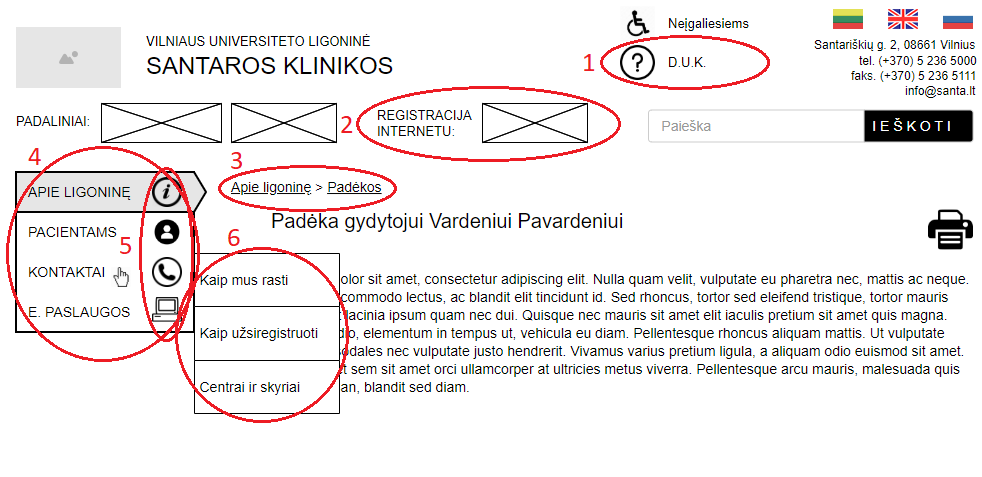
\includegraphics[scale=0.65]{img/NavigacijosPrototipas}
    \caption{Navigacijos sistemos maketas su pataisymais}
    \label{img:NavigacijosPrototipas}
\end{figure}

\section{Reikalavimai ir projektavimo gairės}
Siekiant ištaisyti defektus informacijos architektūroje ir paieškos sistemoje reikia apibrėžti reikalavimus, kurie išspręstų defektų priežastis. Tuo tikslu surašyti funkciniai ir nefunkciniai reikalavimai paieškos sistemai ir projektavimo gairės navigacijos ir informacijos architektūrai. Reikalavimai remiasi naudotojų poreikiais, gairėmis ir euristikomis, kurios buvo naudotos defektams surasti (lentelės \ref{PaieškosLentelėPrad}, \ref{NavigacijosirIALentelėPrad} ir \ref{EuristikųLentelėPrad}).

\subsection{Funkciniai reikalavimai paieškos sistemai}
\begin{enumerate}
	\item Paieškos rezultatų puslapis turi parodyti, atliktos užklausos įvestį ir paieškos nustatymus (frazės tikslumas, rikiavimas, filtravimas, kiek puslapių rodoma)
	\item Paieškos rezultatai turi turėti puslapio pavadinimą ir paryškintą teksto ištrauką, kuri atitinką užklausą
	\item Paieškos rezultatai turi būti reitinguojami pagal atitikimą užklausai
	\item Paieškos rezultatų puslapis turi parodyti, kiek rezultatų gražinta, ir turi leisti nustatyti kiek rezultatų parodyti per puslapį
	\item Paieškos rezultatų puslapis turi leisti nustatyti kaip tiksliai rezultatai turi atitikti užklausos įvestį
	\item Paieškos rezultatų puslapis turi leisti rikiuoti rezultatus pagal populiarumą, datą, abėcėlinę tvarką ir kategoriją
	\item Paieškos rezultatų puslapis turi leisti filtruoti pagal kategoriją
	\item Paieškos sistema turi leisti išsaugoti paieškos nustatymus
	\item Paieškos sistema turi automatiškai patikrinti rašybą, ieškoti daugiaskaitinių formų ir sinonimų
	\item Jei paieška negražina rezultatų, turi būti pasiūlomi pakeitimai užklausai pagerinti
	\item Įvedus tuščią užklausą atsidaro paieškos rezultatų puslapis be rezultatų
	\item Paieškos sistemos nustatymai pritaikyti dažnoms užklausoms
	\item Paieškos rezultatų puslapyje turi būti patarimai, kaip naudoti paiešką
	\item Paieškos rezultatų puslapis turi nerodyti pasikartojančių rezultatų
	\item Paieška turi apimti visą tinklapio turinį
	\item Nukopijavus atliktos paieškos rezultatų puslapio adresą turi būti galima kartoti paiešką
	\item Paieškos rezultatų puslapis turi parodyti naudingą informaciją apie informaciją, kaip dokumento dydis, dokumento sukūrimo data ir failo tipas
	\item Kai paieška užtrunka ilgiau nei sekundę, turi būti parodomi ženklai, kad vyksta paieškos procesas
\end{enumerate}

\subsection{Nefunkciniai reikalavimai paieškos sistemai}
\begin{enumerate}
	\item Pagrindinė paieška turi būti sudaryta tik iš vieno įvedimo lauko ir mygtuko, operuojama pele arba klaviatūra
	\item Paieškos laukas turi leisti įvesti bent 64 simbolių ilgio užklausą
	\item Paieškos laukas turi būti viršuje dešinėje
\end{enumerate}

\subsection{Projektavimo gairės navigacijos ir informacijos architektūrai}
\begin{enumerate}
	\item Navigacijos sistema turi leisti pasiekti visus puslapius
	\item Navigacija turi leisti peržiūrėti visus jos elementus neatidarant kito puslapio
	\item Internetinė registracija pas gydytoją (nuoroda į sergu.lt) turi būti pasiekiama iš bet kurio puslapio
	\item Turi būti tinklapio žemėlapis, kuriame matyti tinklapio turinio apžvalga
	\item Turi būti dažnai užduodamų klausimų puslapis, kuriame paaiškinama kaip naudotis tinklapiu
	\item Turi būti režimas neįgaliesiems, leidžiantis padidinti teksto šriftą, pakeisti puslapio spalvas prastai matantiems
	\item Visuose puslapiuose, išskyrus pagrindinį, turi būti rodomas nukeliautas kelias per paryškintus navigacijos meniu skyrius ir nuorodas į tėvinius skyrius
	\item Turi būti matomi spalvos arba formos pasikeitimai, kai naudotojas užveda kursorių and kažko paspaudžiamo (ne tik kursoriaus pasikeitimai)
	\item Nuoroda į pagrindinį puslapį turi būti puslapio viršuje
	\item Nuolatiniai puslapiai sudėti į navigacijos meniu, nuoroda registracijai pas gydytoją internetu puslapio viršuje
	\item Navigacijos skyriai išrikiuoti pagal naudojimo dažnį, bet taip kad svarbūs skyriai išliktų netoli viršaus
	\item Navigacijos tėviniai skyriai turi būti susieti su paveiksliukais
	\item Navigacijos sistema turi būti plati ir sekli (daug meniu elementų), o ne gili (daug meniu lygių)
	\item Navigacijos meniu turi būti matomas visuose puslapiuose
	\item Navigacijos skirtukai turi atrodyti paspaudžiami
	\item Tinklapio žemėlapį turi būti galima pasiekti iš bet kurio puslapio
	\item Tinklapio žemėlapis turi suteikti glaustą tinklapio apžvalgą
	\item Kategorijų pavadinimai turi tiksliai apibūdinti informaciją viduje
	\item Nuorodos ir navigacijos pavadinimai turi susidaryti iš raktinių žodžių, kurių naudotojai ieškos bandydami atlikti užduotį
	\item Terminologija ir susitarimai (kaip nuorodų spalvos) turi atitikti bendrą interneto naudojimą
	\item Tekste yra nuorodos į susijusius skyrius (gali būti skirtingi nuorodų pavadinimai)
	\item Visuose puslapiuose galima grįžti atgal paspaudus naršyklės „atgal“ mygtuką
	\item Kai puslapis sukuria naujus langus, jie turi būti nedideli ir lengvai uždaromi
\end{enumerate}

\subsection{Papildoma sistemos projektavimo gairė}
Autorius pastebėjo, kad sistema lėtai atidarinėja puslapius ir atlieka paieškas, šie veiksmai užtrunka arti 3 sekundžių. Šis sistemos bruožas labai gadina naudotojo patirtį ir turėtų būti sumažintas iki 1 sekundės ar mažiau tam, kad sistema nevargintų naudotojo.


\section{Informacijos architektūros projektavimas}
\subsection{Informacijos architektūra}
Prieš gilinantis į informacijos architektūros projektavimą reikia patikslinti, kas yra informacijos architektūra (sutrumpintai IA). Autoriai Louis Rosenfeld ir Peter Morville knygoje „Information Architecture for the World Wide Web“ pateikia kelis apibrėžimus šiai plačiai sąvokai apibūdinti. Dvi iš jų puikiai tinka šio darbo kontekste, IA yra: 1. organizavimo, kategorizavimo ir navigacijos schemų rinkinys informacinei sistemai 2. informacinės edvės struktūrinė architektūra palengvinanti užduočių vykdymą ir leidžianti intuityviai rasti turinį \cite{IADefinition}.

\subsection{Turinio išdėstymas}
Vienas iš informacijos architektūros aspektų yra turinio išdėstymas, kaip sudėlioti turinį, kad šis lankytojui jaustųsi natūralus ir būtų lengva rasti ko ieško. Svetainėje autorius rado tris pagrindinius puslapių tipus, kurie turi šiek tiek skirtingą turinio išdėstymą: pagrindinis puslapis, turinio puslapis ir paieškos puslapis (\ref{img:PagrindinisPuslapis}, \ref{img:TurinysPuslapis} ir \ref{img:PaieškaPuslapis} pav.). Pagrindinio puslapio centre esantis elementas su slankiojančiais pranešimais pavadintas fasadu.

Paieškos laukas yra viršuje dešinėje, tai atitinka 1.2.3 reikalavimą. Pagrindinio puslapio dabartinis meniu (\ref{img:PuslapioArchPagrindinisDabartinis} pav.) yra nestandartinio pavidalo ir kitoje vietoje nei visuose kituose puslapiuose, tai gali klaidinti naudotojus. Vietoje to būtų galima įdėti vertikalų meniu, kuris yra kituose puslapiuose, arba navigaciją perdaryti viršuje į horizontalųjį meniu. Šie du sprendimai yra dažniausiai pasitaikančios meniu formos ir yra daug argumentų kada reikėtų rinktis vieną arba kitą, vienintelis aiškus sutarimas yra, kad sprendimas priklauso nuo konteksto. Vienas „naudotojo patirties“ (angliškai „user interface“, toliau „UI“) ekspertas rašo, kad vertikali navigacija geriau tinka, kai visi skyriai panašiai dažnai naudojami\cite{TopVsLeftNav}. Kadangi žmonės skenuoja informaciją iš kairės į dešinę, horizontalaus meniu pirmieji skyriai labiau akcentuojami, negu tolimesni. Skenavimas iš viršaus į apačią netaip stipriai akcentuoja viršutinius skyrius ir dėl to vertikalaus meniu skyriai išlieka panašiai pastebimi. Vertikalų meniu žmonės gali greičiau peržiūrėti\cite{TopVsLeftNav}. Kitas šio eksperto pastebėjimas, kad vertikalų meniu lengviau plėsti\cite{TopVsLeftNav}. Tai galima lengvai paaiškinti, visada galima slinkti puslapį į apačią, bet slinkimas į šonus yra nepageidaujamas. Dar viena UI ekspertė turi labai panašų požiūrį į šių sprendimų privalumus ir trūkumus\cite{TopVsLeftNav2}. Vienas jos šaltinių „Patternfly“ rašo, kad vertikali navigacija tapo populeresnė, kai naudotojai pradėjo naudoti plačiaekranius monitorius ir tapo galima naudoti daugiau vertikalios vietos\cite{LeftNav}. Vertikalus meniu leidžia kiekvienam skyriui suteikti daugiau vietos ir netgi pridėti paveiksliuką (reikalavimas 1.3.12) neapgriozdinant meniu, kas leidžia pagerinti skyrių atpažinimą. Galiausiai, vertikalų meniu lengviau perkelti ant mobilaus ekrano, nes jį galima integruoti beveik be pakeitimų.

\pagebreak
\begin{figure}[htb]
    \centering
    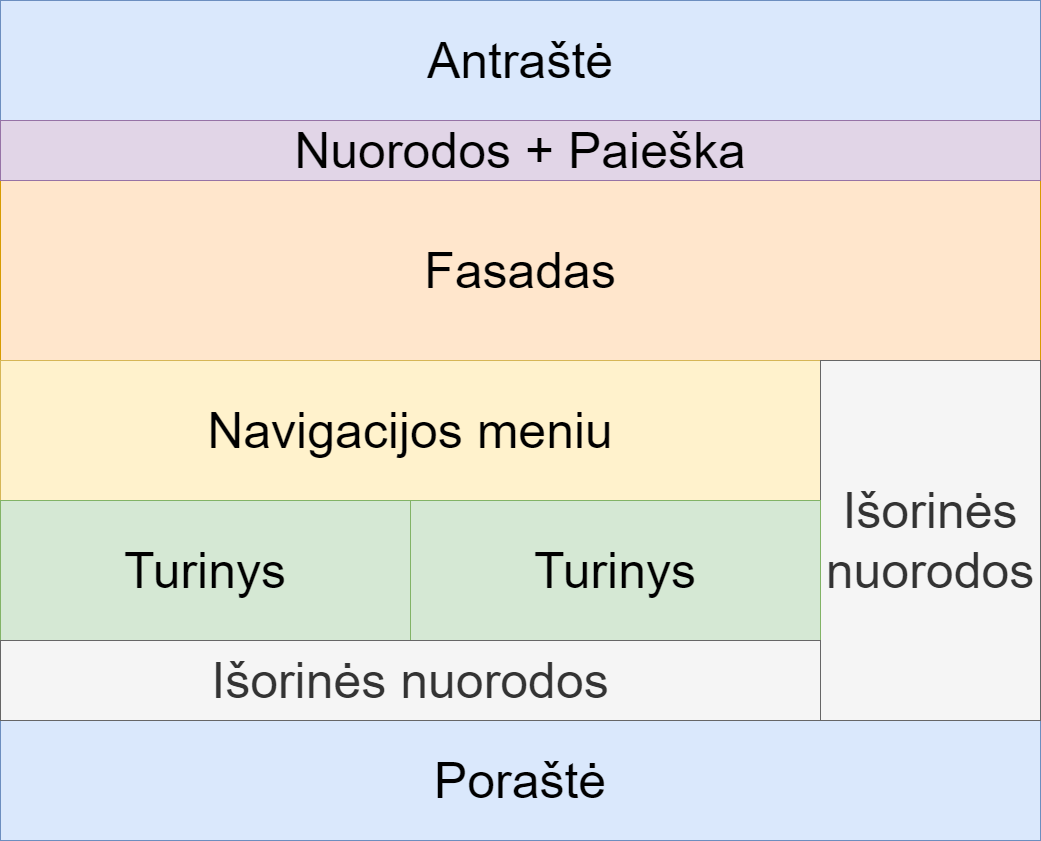
\includegraphics[scale=0.25]{img/PuslapioArchPagrindinisDabartinis}
    \caption{Pagrindinio puslapio dabartinis išdėstymas}
    \label{img:PuslapioArchPagrindinisDabartinis}
\end{figure}

%Navigacija pagrindiniame puslapyje yra virš raukšlės (angliškai „above the fold“), kur į ją atkreips dėmesį daug daugiau vartotojų \cite{Scrolling}

%Elementų išdėstymo schemos kiekvienam puslapio tipui pavaizduoti \ref{img:PuslapioArchPagrindinis}, \ref{img:TurinysArch} ir \ref{img:PaieškaArch} paveiksluose.

\begin{figure}[htb]
\centering
\begin{minipage}{.5\textwidth}
  \centering
  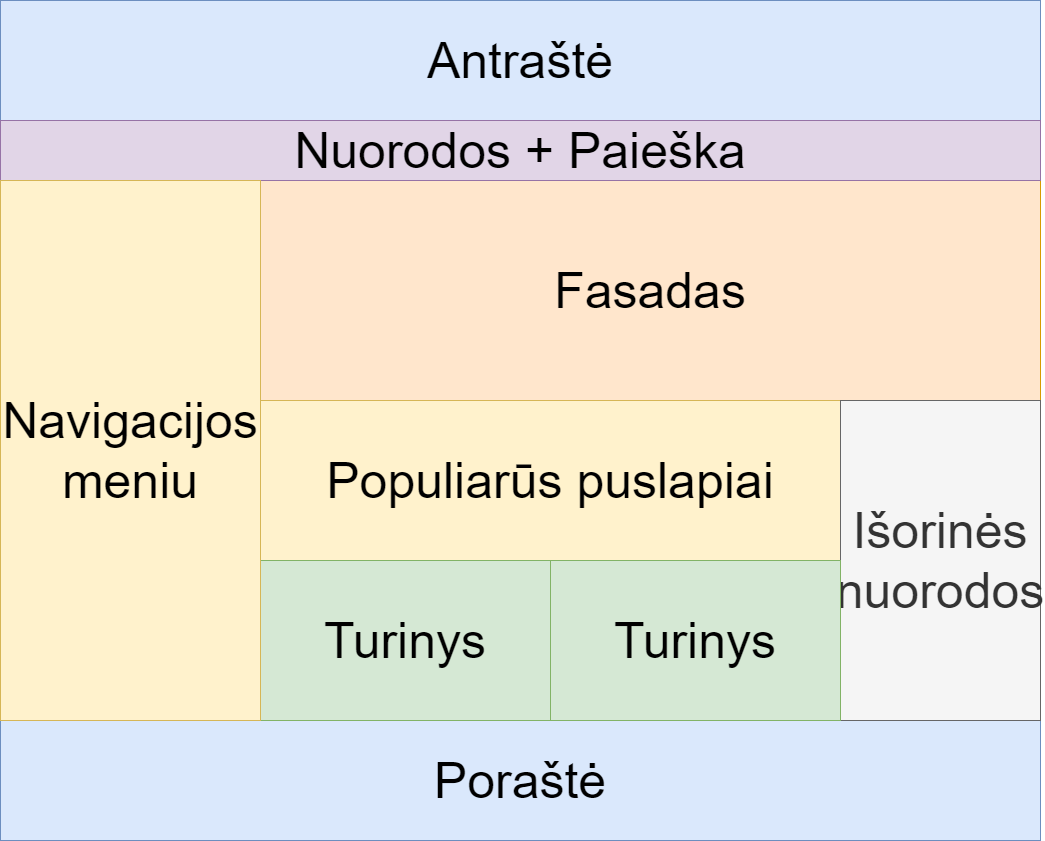
\includegraphics[width=0.9\linewidth]{img/PuslapioArchPagrindinis}
  \captionof{figure}{Pagrindinio puslapio išdėstymas A}
  \label{img:PuslapioArchPagrindinis}
\end{minipage}%
\begin{minipage}{.5\textwidth}
  \centering
  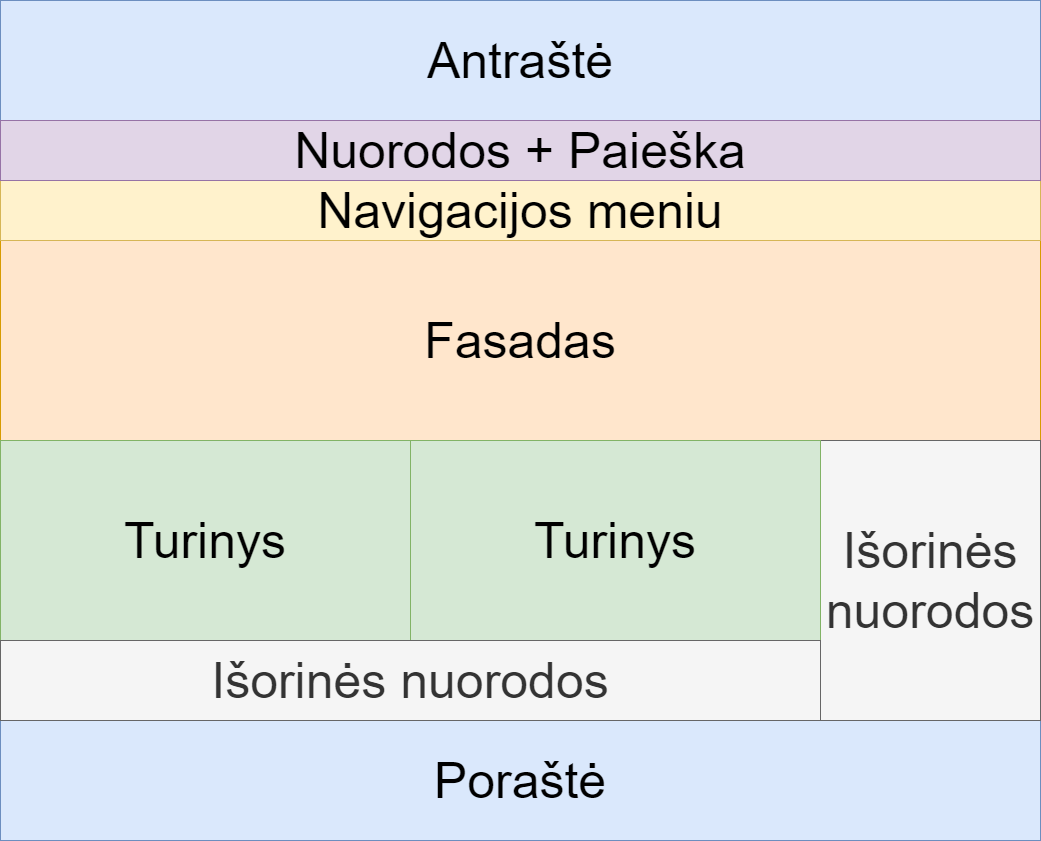
\includegraphics[width=0.9\linewidth]{img/PuslapioArchPagrindinisHorizontalus}
  \captionof{figure}{Pagrindinio puslapio išdėstymas B}
  \label{img:PuslapioArchPagrindinisHorizontalus}
\end{minipage}
\end{figure}

Autoriaus nuomone, šio tinklapio lankytojai be registracijos (tam jau yra numatyta vieta puslapyje) gali vienodai ieškoti informacijos įvairiuose skyriuose: ligoninės adreso, naujienų, pacientų priėmimo tvarkos ir kitų. Šiuo atveju vertikali navigacija labiau tinka, nes ji neturi didelės įtakos skyrių pastebimumui ir vartotojas gali lengvai atsirinkti ko jam reikia. Dėl visų išvardintų vertikalios navigacijos privalumų autorius mano, kad tinklapio pagrindiniam puslapiui geriausiai tiktų \ref{img:PuslapioArchPagrindinis} pav. architektūra.

\begin{figure}[htb]
\centering
\begin{minipage}{.5\textwidth}
  \centering
  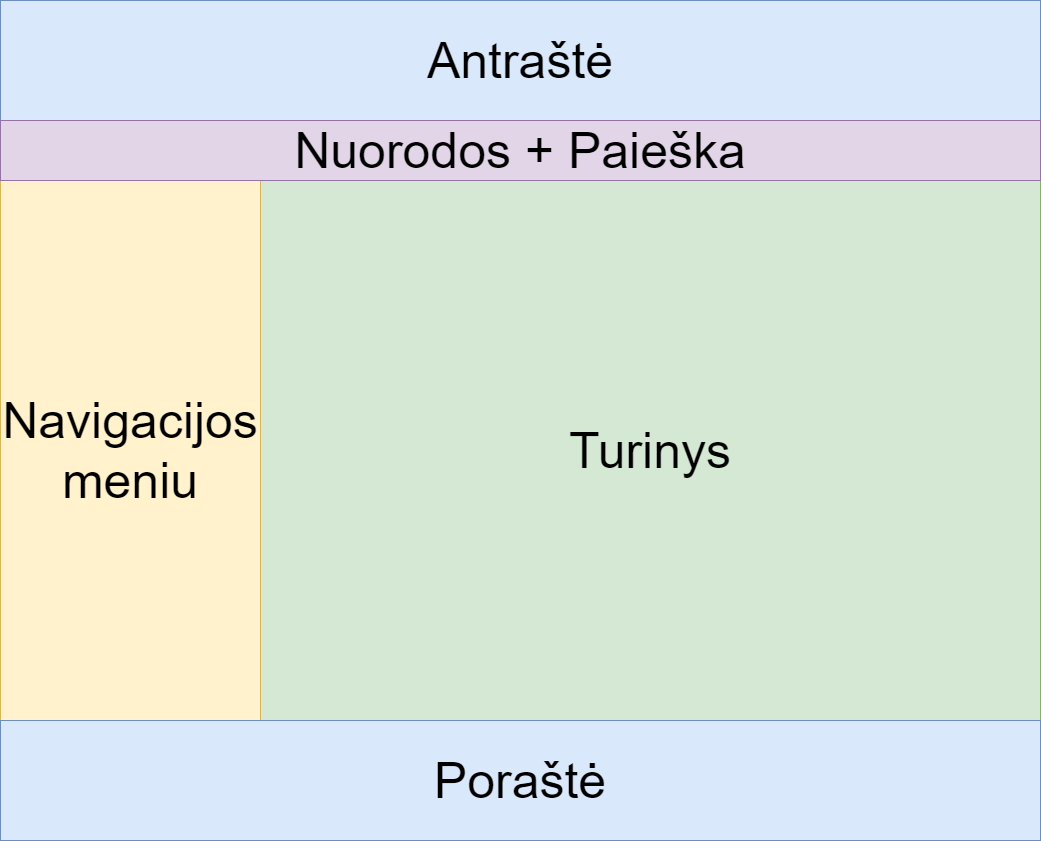
\includegraphics[width=0.9\linewidth]{img/PuslapioArchTurinys}
  \captionof{figure}{Turinio puslapio išdėstymas}
  \label{img:TurinysArch}
\end{minipage}%
\begin{minipage}{.5\textwidth}
  \centering
  \includegraphics[width=0.9\linewidth]{img/PuslapioArchPaieška}
  \captionof{figure}{Paieškos puslapio išdėstymas}
  \label{img:PaieškaArch}
\end{minipage}
\end{figure}

Kituose puslapiuose yra standartinis išdėstymas. Navigacija kairėje kaip ir pagrindiniame puslapyje, tai palengvina naudotojui atsiminti ir priprasti prie navigacijos. Kitiems puslapio elementams nėra specifinių reikalavimų, čia nebuvo rasta defektų, taigi galima jų nekeisti.

\pagebreak
\subsection{Navigacijos meniu}
Tiriant navigacijos ir informacijos architektūros panaudojamumą buvo rasta, kad navigacija per daug gili (\ref{NavigacijosirIALentelėPrad}.4 defektas), yra pernelyg sudėtinga (\ref{NavigacijosirIALentelėPrad}.5 defektas) ir kategorijų pavadinimai neapibūdina informacijos viduje (\ref{NavigacijosirIALentelėPrad}.12 defektas), nes į kategoriją sudėta per daug elementų. Siekiant patenkinti projektavimo gaires (1.3.13, 1.3.18) reikėjo pataisyti navigacijos skyrių išdėstymą.

\begin{figure}[htb]
    \centering
    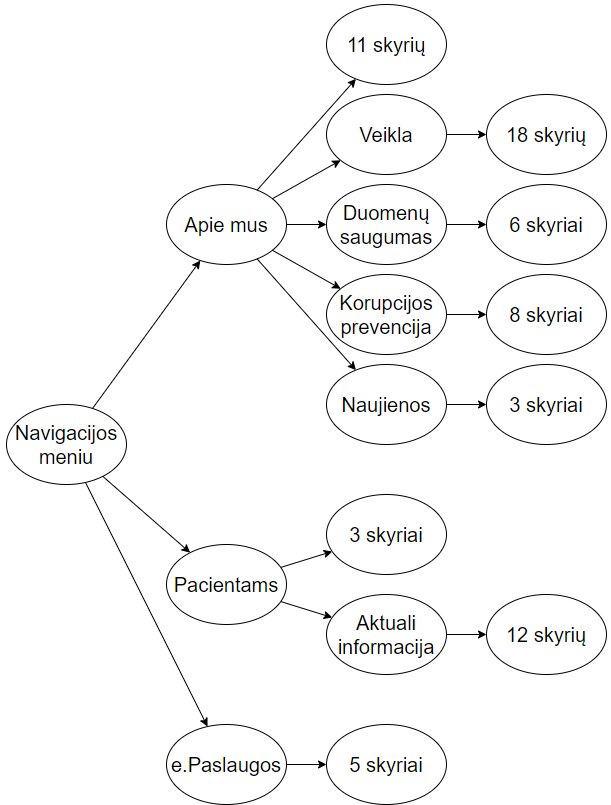
\includegraphics[scale=0.8]{img/NavigacijosMeniuDabartinis}
    \caption{Dabartinio navigacijos meniu diagrama}
    \label{img:NavigacijosMeniuDabartinis}
\end{figure}

\pagebreak
Dabartinės sistemos navigacijos meniu pavaizduotas diagramoje (\ref{img:NavigacijosMeniuDabartinis} paveikslas). Šio meniu pirmame lygyje tik trys skyriai, taigi iš šio lygio nedaug galima sužinoti apie tinklapio turinį. Į skyrių „Apie mus“ sudėti 15 skyrių, o 4 iš jų rodo į trečią lygį, iš viso „Apie mus“ skyrius turi 46 vaikinius skyrius, daug daugiau nei bet kuris kitas skyrius. Vienas iš vaikinių skyrių yra nuoroda į paiešką, autoriaus nuomone tai yra perteklinis skyrius, kurio galima atsisakyti, nes paieška matoma visuose puslapiuose. Po pakeitimų gautas navigacijos meniu pavaizduotas \ref{img:NavigacijosMeniuPakeistas} paveiksle.

Atlikti pakeitimai navigacijos meniu:
\begin{enumerate}
	\item Panaikintas trečias lygis perkeliant visus trečio lygio skyrius ir jų tėvinį skyrių vienu lygiu aukštyn
	\item Nauji pirmo lygio skyriai surūšiuoti pagal jų svarbą naudotojui
	\item Panaikintas skyrius nurodantis į paiešką
	\item Panaikintas skyriaus „Patalpų nuoma“ duplikatas
	\item Skyriaus „Pacientams“ vaikiniai skyriai apkeisti vietomis su skyriaus „Aktuali informacija“ vaikiniais skyriais (paryškinti spalvomis)
	\item Panaikintas „Apie mus“ skyriaus identiško pavadinimo vaikinis skyrius, kad suvienodinti veikseną tarp skyrių
\end{enumerate}

\begin{figure}[htb]
    \centering
    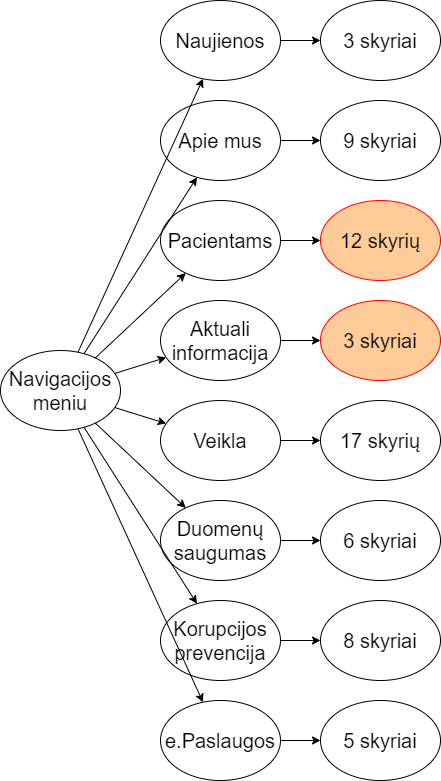
\includegraphics[scale=0.65]{img/NavigacijosMeniuPakeistas}
    \caption{Pakeisto navigacijos meniu diagrama}
    \label{img:NavigacijosMeniuPakeistas}
\end{figure}

\section{Svetainės prototipo kūrimo procesas}


\sectionnonum{Rezultatai ir išvados}
%Šiame darbe išskirti funkciniai ir nefunkciniai reikalavimai paieškai, navigacijos ir informacijos architektūros projektavimo gairės, parinkti tinklapio architektūros maketai, suprojektuotas navigacijos meniu ir aprašytas bendras sistemos serverio architektūros modelis.

%Formuluojant reikalavimus iš gairių autorius pastebėjo, kad nevisiems defektams prasminga rašyti reikalavimus, kadangi nevisi defektai yra aktualūs gerinamai sistemai, o kai kurie turi bendrą iškilimo priežastį. Atliekant vertikalios ir horizontalios navigacijos palyginimą išsiaiškinta, kad vertikali geriau tinka, kai meniu labai platus ir yra naudojamas kaip orientacinis elementas, ne tik informacijos paieškos elementas. Taip pat paaiškėjo, kad horizontalų meniu gerai naudoti, kai kažkurie skyriai daug dažniau naudojami, ir jį naudojant galima užimti mažiau vietos navigacijai. Projektuojant navigacijos meniu autorius pastebėjo, kad net sutalpinus daug skyrių į meniu, informacija gali būti lengvai surandama, jeigu viskas tvarkingai surūšiuota.

%Rezultatų ir išvadų dalyje turi būti aiškiai išdėstomi pagrindiniai darbo
%rezultatai (kažkas išanalizuota, kažkas sukurta, kažkas įdiegta) ir pateikiamos
%išvados (daromi nagrinėtų problemų sprendimo metodų palyginimai, teikiamos
%rekomendacijos, akcentuojamos naujovės).

\printbibliography[heading=bibintoc, title=Šaltiniai]  % Šaltinių sąraše nurodoma panaudota
% literatūra, kitokie šaltiniai. Abėcėlės tvarka išdėstomi darbe panaudotų
% (cituotų, perfrazuotų ar bent paminėtų) mokslo leidinių, kitokių publikacijų
% bibliografiniai aprašai. Šaltinių sąrašas spausdinamas iš naujo puslapio.
% Aprašai pateikiami netransliteruoti. Šaltinių sąraše negali būti tokių
% šaltinių, kurie nebuvo paminėti tekste. Šaltinių sąraše rekomenduojame
% necituoti savo kursinio darbo, nes tai nėra oficialus literatūros šaltinis.
% Jei tokių nuorodų reikia, pateikti jas tekste.

% \sectionnonum{Sąvokų apibrėžimai}
%\sectionnonum{Santrumpos}
%Sąvokų apibrėžimai ir santrumpų sąrašas sudaromas tada, kai darbo tekste
%vartojami specialūs paaiškinimo reikalaujantys terminai ir rečiau sutinkamos
%santrumpos.

\appendix  % Priedai
% Prieduose gali būti pateikiama pagalbinė, ypač darbo autoriaus savarankiškai
% parengta, medžiaga. Savarankiški priedai gali būti pateikiami ir
% kompaktiniame diske. Priedai taip pat numeruojami ir vadinami. Darbo tekstas
% su priedais susiejamas nuorodomis.
\sectionnonumnocontent{Trys puslapių tipai}

\begin{figure}[H]
    \centering
    
\includegraphics[scale=0.65]{img/Pagrindinis}
    \caption{Pagrindinis puslapis}
    \label{img:PagrindinisPuslapis}
\end{figure}
\begin{figure}[H]
    \centering
    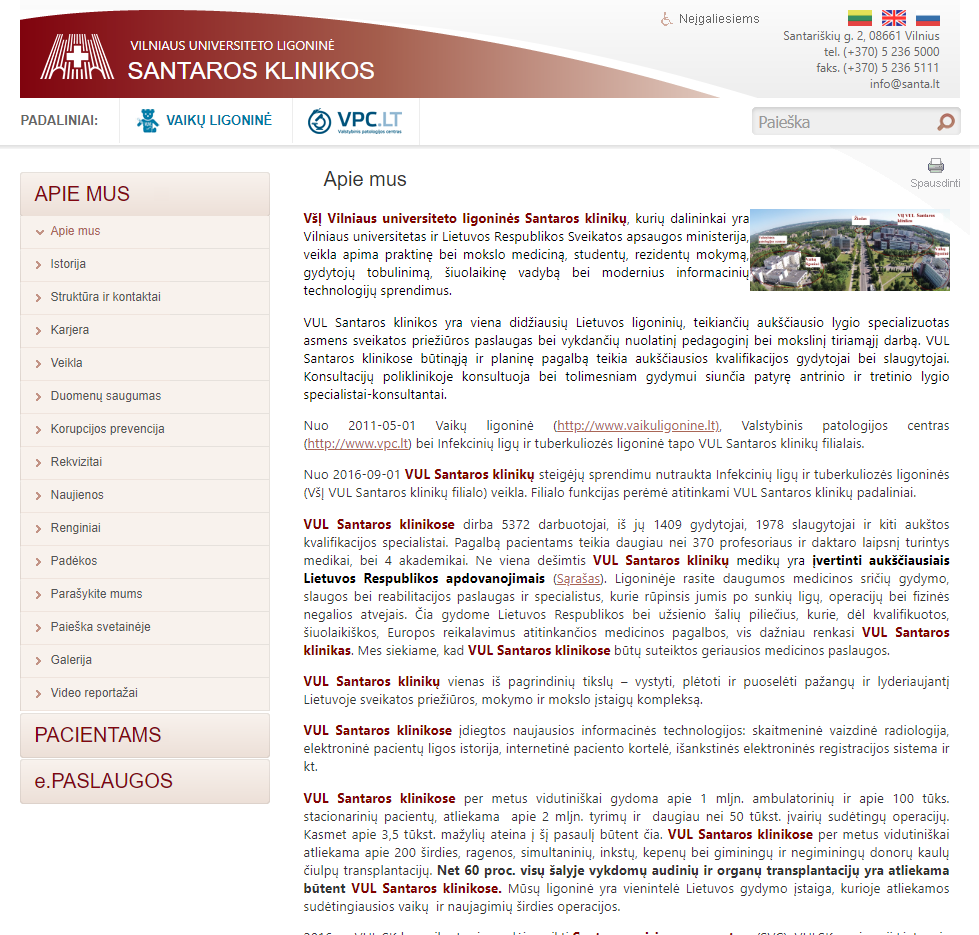
\includegraphics[scale=0.65]{img/Turinys}
    \caption{Turinio puslapis}
    \label{img:TurinysPuslapis}
\end{figure}
\begin{figure}[H]
    \centering
    \includegraphics[scale=0.65]{img/Paieška}
    \caption{Paieškos puslapis}
    \label{img:PaieškaPuslapis}
\end{figure}

\sectionnonumnocontent{Prototipo paleidimo instrukcija}
Bakalaurinis darbas įkeltas į GitHub repozitoriją adresu: \textbf{https://github.com/Steror/Bakalaurinis-darbas}
Prototipas įkeltas adresu: \textbf{https://github.com/Steror/Bakalaurinis-darbas/tree/master/Tinklapis/client}

Norint pasileisti prototipą reikia:
\begin{enumerate}
	\item Parsisiūsti prototipą (https://github.com/Steror/Bakalaurinis-darbas/tree/master/Tinklapis/client)
	\item Parsisiūsti ir įrašyti Node Package Manager (toliau NPM) pagal savo kompiuterio platformą (https://nodejs.org/en/download/)
	\item Įsirašyti naujausią Angular CLI naudojant NPM (per Windows į komandinę eilutę reikia įrašyti: „npm install -g @angular/cli@latest“)
	\item Atsidaryti komandinę eilutę prototipo aplankale (per Windows į komandinę eilutę reikia įrašyti: „cd <kelias>/client“, kur vietoj <kelias> reikia įrašyti kelią iki aplanko)
	\item Sukompiliuoti ir paleisti prototipą naudojant Angular CLI (per Windows į komandinę eilutę reikia įrašyti: „ng serve -o“)
	\item Jeigu prototipas sėkmingai paleistas, adresu http://localhost:4200/ turėtų užkrauti puslapį
\end{enumerate}

\end{document}
